\documentclass[hyperref=colorlinks]{beamer}
\mode<presentation>
\usetheme{iclpt}
\setbeamertemplate{navigation symbols}{}
\setbeamertemplate{headline}{
  \begin{beamercolorbox}[leftskip=.2cm,rightskip=.2cm,topskip=.2cm,ht=1.1cm,dp=0.1cm,wd=\textwidth]{institute in head/foot}
    
\includegraphics[height=1cm]{icl.pdf}
    \hfill
%    \includegraphics[height=1cm]{../Pics/ATLAS-Logo-Square-Blue-RGB.png}
%    
\includegraphics[height=1cm]{../Pics/CMS-Color.pdf}
    
\includegraphics[height=1cm]{TalkPics/t2k_logo_large.png}

%??put t2k logo here
  \end{beamercolorbox}
}
\setbeamertemplate{footline}{
  \begin{beamercolorbox}[ht=.35cm,dp=0.2cm,wd=\textwidth,leftskip=.3cm]{author in head/foot}%
    \begin{minipage}[c]{5cm}%
      \usebeamerfont{author in head/foot}
      \insertshortauthor 
      \insertshorttitle
    \end{minipage}\hfill%
    \hfill
    \insertframenumber{} / \ref{lastframe}
    %\hfill
    \begin{minipage}{6cm}
      \hfill
      %\insertshorttitle
    \end{minipage}
  \end{beamercolorbox}%
}

\definecolor{beamer@icdarkblue}{RGB}{0,51,102}
\definecolor{beamer@icmiddleblue}{RGB}{0,82,150} 
\definecolor{beamer@iclightblue}{RGB}{200,212,232}
\definecolor{beamer@icmiddlered}{RGB}{204,51,0}
\definecolor{beamer@iclightred}{RGB}{232,212,32}

\usepackage{tikz}
\usetikzlibrary{arrows,shapes,backgrounds}
\usepackage{color}
\usepackage{tabularx,colortbl}
\usepackage{graphicx}
\usepackage{pdfpages}
\usepackage{feynmp}
\usepackage{rotating}
\usepackage{moresize}
\usepackage{slashed}
\usepackage{xcolor,colortbl}
\DeclareGraphicsRule{*}{mps}{*}{}
\hypersetup{colorlinks=false}

\title[2D vs 1D yields]{\vspace{-0.2cm} 2D vs 1D yields}
\author[P. Dunne]{Patrick Dunne - Imperial College London}
\titlegraphic{
  \vspace{-0.4cm}
}
\date{}
\begin{document}
\tikzstyle{every picture}+=[remember picture]
\tikzstyle{na} = [baseline=-.5ex]
\begin{fmffile}{t2ktemplatefeyndiags}


  %TITLE PAGE
  %20 mins + 5 questions
  \section{Title}
  \begin{frame}
    \titlepage
  \end{frame}

  \begin{frame}
    \frametitle{Overview}
    \begin{block}{}
        \scriptsize
        \begin{itemize}
        \item Checking the effect of moving from 1D bins in $E_{rec}$ to 2D bins in $E_{rec}$-$\theta$ for the $\nu_{e}$ sample on MaCh3
        \item[-] $\nu_{\mu}$ sample still using 1D $E_{rec}$ bins.
        \item[-] Valor splines used for $\nu_{e}$
        \item Have compared rates from and kinematic distributions from 2D with valor
      \end{itemize}
        \begin{tabular}{|c||c|c|c|c|c|c|} 
          \hline
          & $\nu_{\mu}$ & $\nu_{e}$ & $\bar{\nu}_{\mu}$ & $\bar{\nu}_{e}$ & $\nu_{e}$ signal & $\bar{\nu}_{e}$ signal \\ 
          \hline
          \textbf{1D}  & 1.468 & 3.271 & 0.069 & 0.144 & 21.544 & 0.139 \\ 
          \hline
          \textbf{1D Total}& \multicolumn{6}{c|}{26.635} \\
          \hline
          \hline
          \textbf{2D}  & 1.468 & 3.262 & 0.069 & 0.145 & 21.493 & 0.138 \\ 
          \hline
          \textbf{2D Total}& \multicolumn{6}{c|}{26.575} \\
          \hline
        \end{tabular} \\
    \begin{itemize}
      \item Also checked kinematic plots with valor bin by bin
      \item[-] Agreement better than 0.1\% in all bins
        %??Rate comparison
      \end{itemize}
    \end{block}
  \end{frame}

  \begin{frame}
    \frametitle{1M step chain contour - appearance}
    \centering
    \begin{block}{}
      \begin{itemize}
      \item As seen by valor 1D and 2D Asimov contours agree well
      \end{itemize}
    \end{block}
    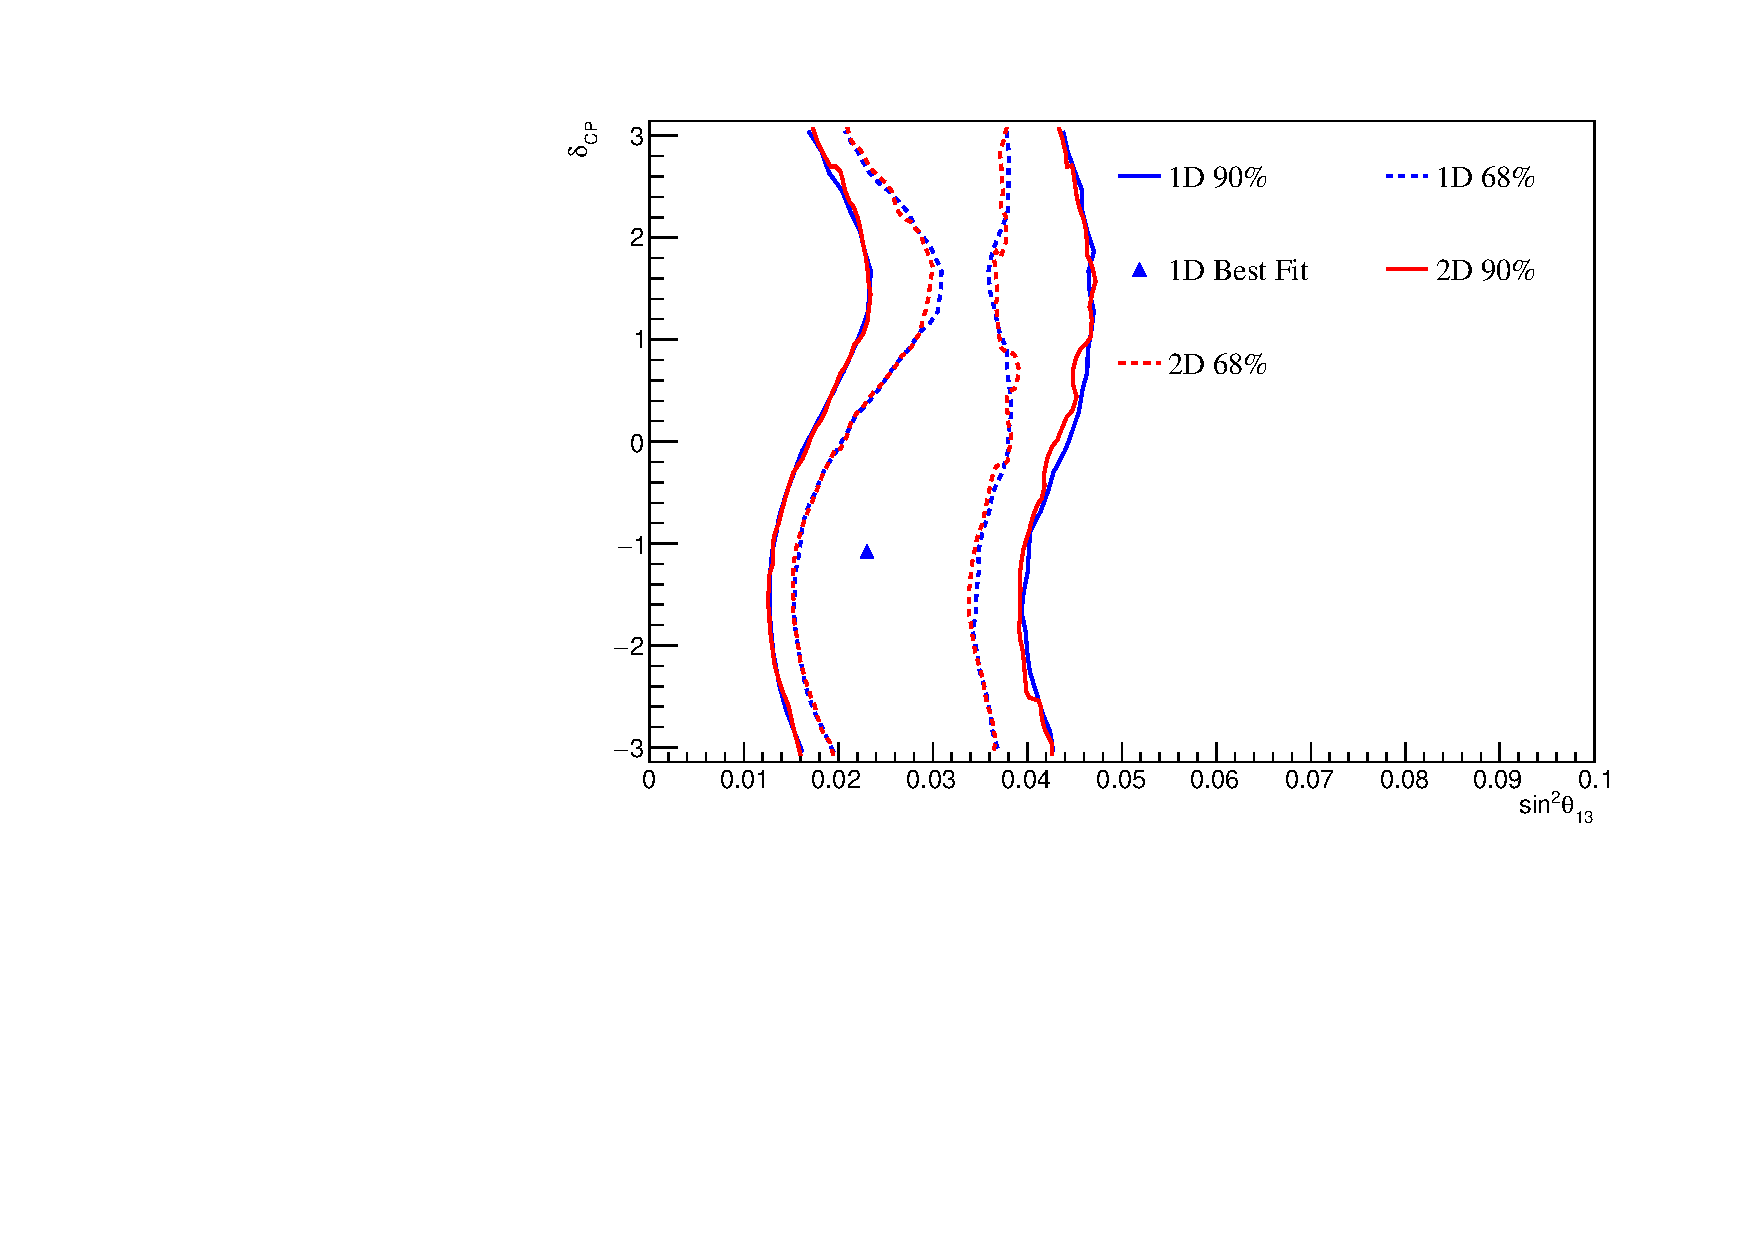
\includegraphics[width=.65\textwidth]{TalkPics/2dvs1d_240516/comparedcontours_app.pdf}
  \end{frame}

  \begin{frame}
    \frametitle{1M step chain contour - disappearance}
    \centering
    \begin{block}{}
      \begin{itemize}
      \item Slight shift seen between 1D and 2D for disappearance contour
      \item[-] under investigation
      \end{itemize}
    \end{block}
    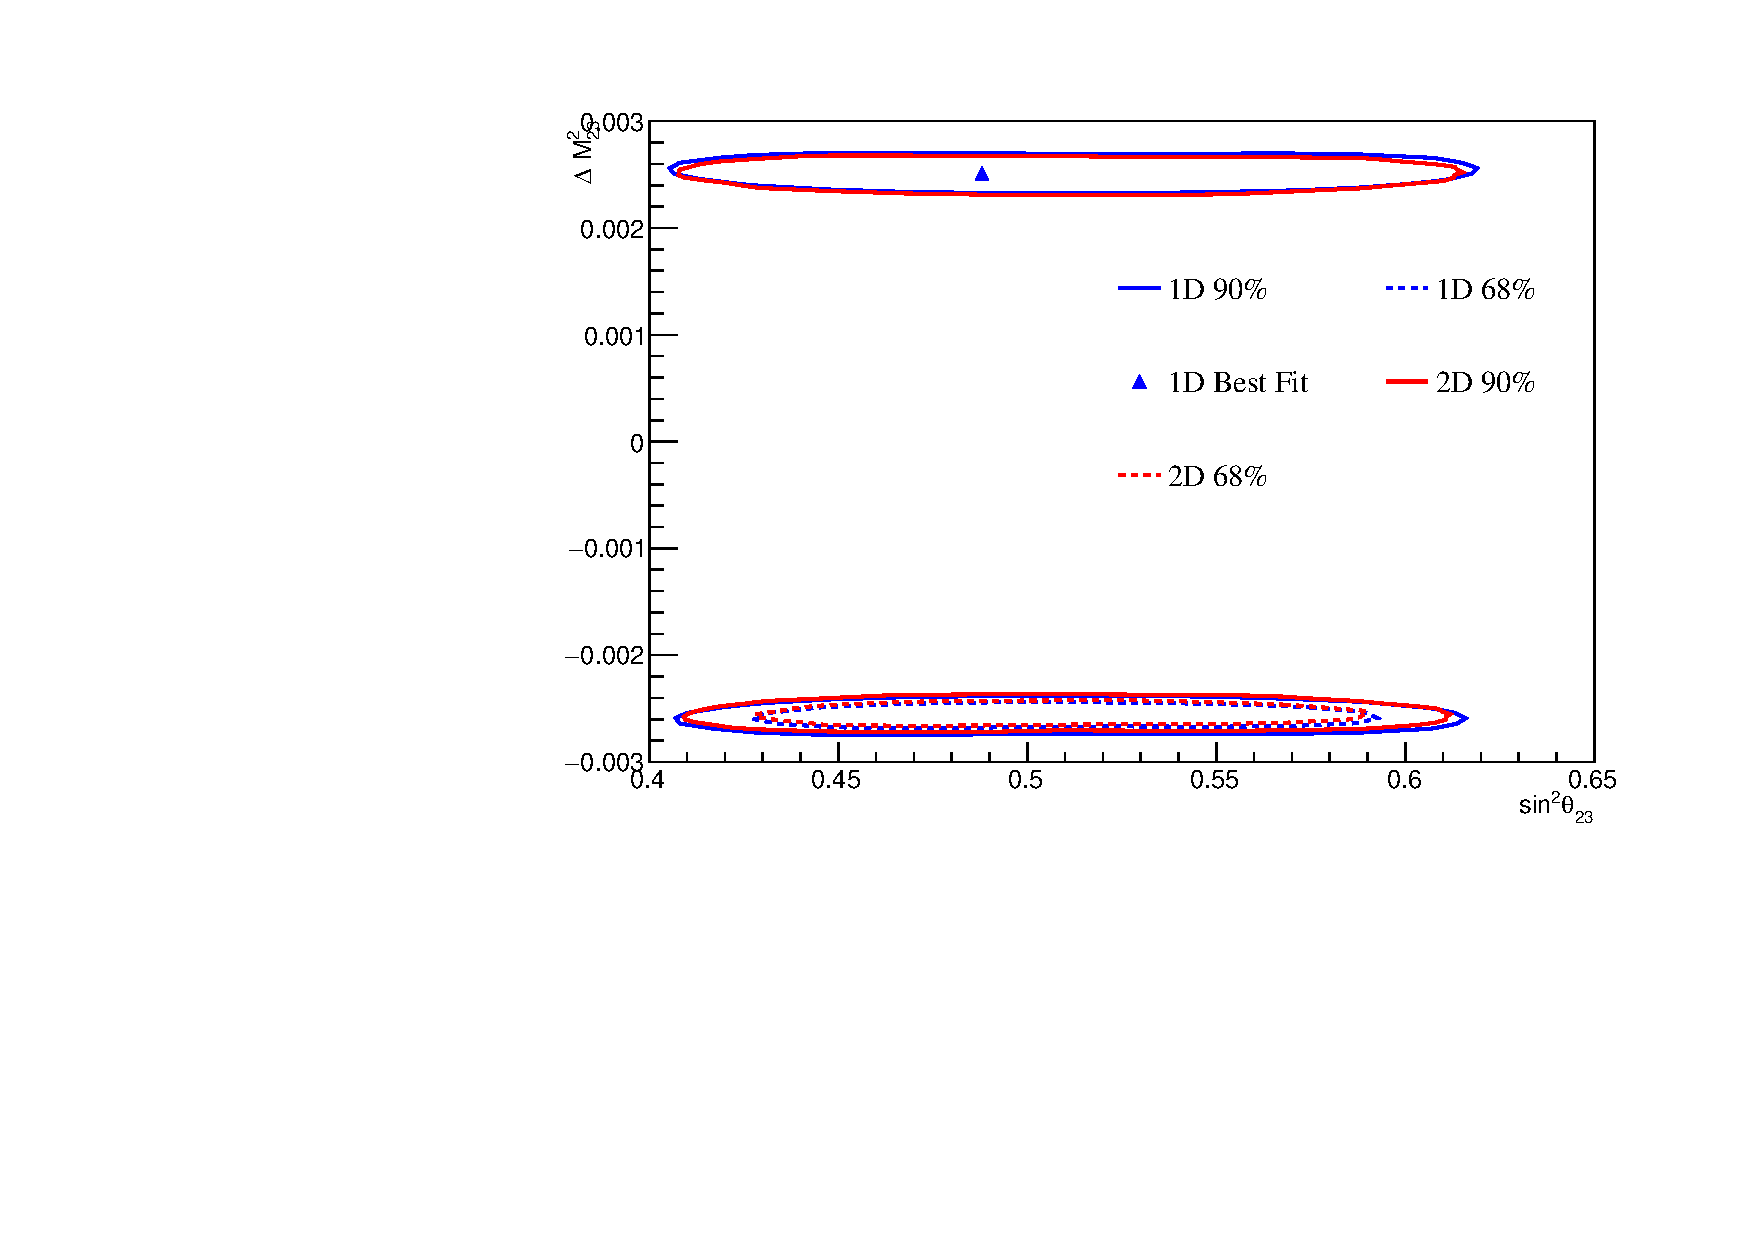
\includegraphics[width=.65\textwidth]{TalkPics/2dvs1d_240516/comparedcontours.pdf}
  \end{frame}


  \begin{frame}
    \frametitle{}
    \label{lastframe}
    \begin{block}{}
      \begin{itemize}
      \item 2D and 1D yields agree very well between MaCh3 and valor
      \item Appearance contours agree well
      \item Shift seen in disappearance contours is under investigation
      \end{itemize}
    \end{block}
  \end{frame}

  %Backup goes here
  
\end{fmffile}
\end{document}

